\subsection{Period 4: Reappearance of a new \change{and weaker} detached haze layer around the Summer Solstice (2015-2017) - $L_s=\ang{75}-\ang{95}$}

The first occurrence of the \change{stable} detached haze in this period was seen on 3$^{rd}$ December 2015
(Fig.~\ref{fig:dhl_2015_2017}a). It
does not at first appear different from the previous sporadic detached haze layers observed in the period 2012-2015. \change{Its signature is very weak, but}, after
this observation, the detached haze was \change{more pronounced and} present in each following observation. The detached haze became stable in time,
similar to the detached haze before the equinox. Therefore, we consider this date as \change{a limit to} the beginning of the
reappearance of the detached haze ($L_s=\ang{74}$). The evolution of the haze during this period is displayed in
Fig.~\ref{fig:dhl_2015_2017}. These observations validate the long awaited reappearance of the detached haze layer,
just before the end of the Cassini mission in September 2017.

\begin{figure*}[!ht]
\plotone{Fig/Lat_beta-2015_2017}
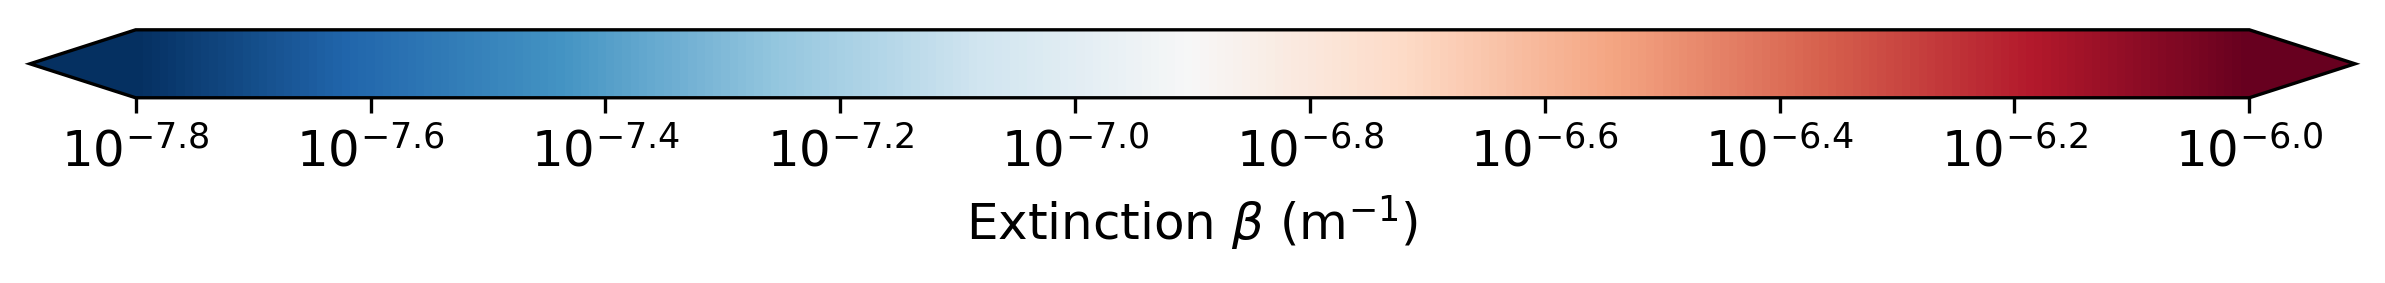
\includegraphics[width=.5\textwidth]{Fig/Extinction_colorbar}
\caption{Same as the figures~\ref{fig:dhl_2004_2008}, \ref{fig:dhl_2008_2012}
and~\ref{fig:dhl_2012_2015} for 6 images taken between 2015 and 2017
($L_s=\ang{75}-\ang{95}$) during the reappearance of the DHL.
The image \textbf{N1884018021\_1} is one of the very last observations of Titan before
the end of the Cassini mission in September 2017.}
\label{fig:dhl_2015_2017}
\end{figure*}

The detached haze layer is not very well defined but it can be perceived at all latitudes
around 490 - 520 km (Fig.~\ref{fig:dhl_2015_2017}a). We notice a contraction
the main haze: the top of the haze dropped by 50 km in January 2016 compared to October 2015
(Fig.~\ref{fig:dhl_2012_2015}d). The main elements of the reappearance (altitude and date) confirm the
predictions made by the general circulation models \citep{Lebonnois2012,Larson2015} and the prediction
reported in \cite{West2011}. The detailed comparison between the observations and the GCM is discussed further
in section 5.

With time, the detached haze layer became more distinct and the zone of depletion more pronounced, especially in the
northern hemisphere (Fig.~\ref{fig:dhl_2015_2017}b). The situation seems to be analogous to an early stage of
the structure observed in 2004 (Fig~\ref{fig:dhl_2004_2008}a, but in the opposite hemisphere).
However, although the detached haze persists in time,
it also settles and almost merges with the main haze in October, 2016 (Fig.~\ref{fig:dhl_2015_2017}c).
In the  following observations (Figs.~\ref{fig:dhl_2015_2017}d and e), we are
witnessing the complex evolution of the newly-formed detached haze that merged with the main layer southward
of \ang{35}N while it remained stable around 450 km northward of \ang{35}N and seems to vanish in May, 2017 rather than settle.
This structure was still observed in the very last image of Titan taken by Cassini just before its final plunge into Saturn
 (Fig.~\ref{fig:dhl_2015_2017}f) in September, 2017.

A secondary detached haze layer appeared in October, 2016 in the southern hemisphere at high altitude (around 520 km \change{ in} Fig.~\ref{fig:dhl_2015_2017}c). Its northern boundary is not well defined. This new structure will be persistent with
time, at planetary scale, up to the end of the Cassini mission but it gradually descended. The results reported by \cite{West2018}
concern the detached haze at the equator only. Although they already revealed a complex behavior of the detached haze layer, the
present observations show a dichotomy between the two hemispheres. The detail of the evolution, the split in a double layer
structure, and the formation and disappearance of several structures were completely unexpected. According to the GCMs mentioned earlier, six years
after equinox, the post-equinoctial circulation was supposed to be already installed with a planetary-scale circulation cell
from the southern hemisphere to the north polar region. Apparently, this is not the case in the observations.

Cassini observations from 2004 to 2017 do not completely cover half a Titan year. The first and last observations
were taken almost at the opposite season, $L_s=\ang{297}$ and \ang{94} respectively (\emph{i.e.} \ang{157} apart).
This prevents direct comparisons of the detached haze at opposite seasonal phases,
although both 2004 and 2017 images are taken more than a season after the previous solstice.
